\documentclass[a4paper,10pt]{ltjsarticle}
\usepackage{luatexja-fontspec}
\usepackage[margin=20mm]{geometry}
\usepackage{graphicx}
\usepackage{booktabs}
\usepackage{xcolor}
\usepackage{url}
\usepackage{float}
\usepackage{caption}
\usepackage{enumitem}
\usepackage{fancyvrb}
\usepackage[hidelinks]{hyperref}
\captionsetup{font=small,labelfont=bf}
\setlist{nosep}
\fvset{fontsize=\small,frame=single,framesep=2mm}
\title{K$^-p$ 散乱イベントディスプレイ（ビーム軌跡つき）\\
\large \texttt{kpsc\_event\_display\_rk.py} 使い方手引き}
\date{2026 年 10 月 1 日}

\begin{document}
\maketitle

\section{概要}
\texttt{kpsc\_event\_display\_rk.py} は、K$^-p$ 散乱解析の 1 イベントを、TPC のトラックとビームの軌跡をあわせて表示する Python スクリプトです。
\texttt{DstTPCHelixTracking}（または \texttt{-Geant4}）の出力と、\texttt{DstKpScattering}（または \texttt{-Geant4}）の出力の 2 つを読み、次の 4 面を 1 枚にまとめます。
\begin{itemize}
\item 3D 表示
\item 上面図（$z$–$x$）
\item 側面図（$z$–$y$）
\item 数値の欄（陽子と K の運動量、弾性散乱からの期待値、mmass など）
\end{itemize}
実データと Geant4（G4）の両方に対応しています。1 イベントを PNG に描くことも、選択条件を満たす $N$ イベントを 1 つの PDF にまとめることもできます。

\begin{itemize}
\item I/O は uproot を使います（ROOT/PyROOT は使いません）。
\item helix の計算（θ の範囲を含む）、座標変換、TPC の枠の描画は、同じ \path{macro/} 内の \path{check_tpc_helix_track_3d.py} から import して再利用しています。helix の描き方はそのマクロと同じです。
\end{itemize}

\section{動作環境}
\begin{itemize}
\item Python 3、uproot、awkward、matplotlib、numpy
\item スクリプトの場所: \path{myanalysis/macro/kpsc_event_display_rk.py}。\path{check_tpc_helix_track_3d.py} に依存するので、この 2 つは同じディレクトリに置きます。
\item 出力はファイルのみです（matplotlib の Agg バックエンドを使うので、画面は開きません）。X11 転送は不要です。
\end{itemize}

\section{入力ファイル}
\begin{table}[H]
\centering\small
\begin{tabular}{lp{0.34\textwidth}p{0.34\textwidth}}
\toprule
 & 実データ & G4 \\
\midrule
\texttt{--helix}（ツリー \texttt{tpc}） & \path{DstTPCHelixTracking} の出力\newline 例: \path{/group/had/sks/Users/sryuta/JPARC2025E72/run03774_TPCHelix.root} & \path{DstTPCHelixTrackingGeant4} の出力（反応の真値ブランチつき）\newline 例: \path{scratch_root/g4_kp_mom735/helix_B1T_truth_n100k.root} \\
\texttt{--kpsc}（ツリー \texttt{kpsc}） & \path{DstKpScattering} の出力\newline 例: \path{root/run03774/run03774_KpScattering_lh2off.root} & \path{DstKpScatteringGeant4} の出力\newline 例: \path{scratch_root/g4_kp_mom735/kpsc_B1T_hon_off_s0_n100k.root} \\
\texttt{--g4} & 付けない & 付ける \\
\bottomrule
\end{tabular}
\end{table}
2 つのファイルは同じイベントを同じ順で含んでいる必要があります（\texttt{--kpsc} は \texttt{--helix} を入力に作ったもの）。
実データのビームの軌跡には kpsc の \texttt{xvp, yvp, zvp}（HSTrack の RK で運んだビームの経路）を使います。
G4 では、kpsc の \texttt{beam\_used\_*}・\texttt{vtx\_*\_true}・\texttt{p\_p\_true} などと、helix の \texttt{beam\_prm\_*}・\texttt{prm\_k\_*} を使います。

\section{基本的な使い方}
\subsection{1 イベントを描く}
実データは run と event で指定します。
\begin{Verbatim}
cd /home/had/sryuta/analyzer/JPARC2025E72/myanalysis/macro
D=/group/had/sks/Users/sryuta/JPARC2025E72
python3 kpsc_event_display_rk.py \
  --helix $D/run03774_TPCHelix.root \
  --kpsc  $D/root/run03774/run03774_KpScattering_lh2off.root \
  --run 3774 --event 560 --out ev_3774_560.png
\end{Verbatim}
G4 は \texttt{event\_number} が一意でないので、kpsc のエントリ番号で指定します（\texttt{--event} でも描けますが、同じ番号が複数あれば最初のエントリになり、その旨を表示します）。
\begin{Verbatim}
G=/group/had/sks/Users/sryuta/JPARC2025E72/scratch_root/g4_kp_mom735
python3 kpsc_event_display_rk.py --g4 \
  --helix $G/helix_B1T_truth_n100k.root \
  --kpsc  $G/kpsc_B1T_hon_off_s0_n100k.root \
  --entry 25 --out ev_g4_25.png
\end{Verbatim}
出力の形式は \texttt{--out} の拡張子で決まります（\texttt{.png}, \texttt{.pdf} など）。

\subsection{選択条件を満たす $N$ イベントを 1 つの PDF にまとめる}
\begin{Verbatim}
D=/group/had/sks/Users/sryuta/JPARC2025E72
O=/home/had/sryuta/JPARC2025E72/results/img/run00000/kpsc_lh2eloss/event_display
python3 kpsc_event_display_rk.py \
  --helix $D/run03774_TPCHelix.root \
  --kpsc  $D/root/run03774/run03774_KpScattering_lh2off.root \
  --n 12 --out $O/kpsc_event_display_data_run03774.pdf
\end{Verbatim}
1 ページに 1 イベントです。\texttt{--skip M} を付けると、選ばれたイベントのうち先頭の $M$ 個を飛ばして次から描きます。

\subsection{オプション一覧}
\begin{table}[H]
\centering\small
\begin{tabular}{lp{0.7\textwidth}}
\toprule
オプション & 意味 \\
\midrule
\texttt{--helix FILE} & helix tracking の出力（必須） \\
\texttt{--kpsc FILE} & KpScattering の出力（必須） \\
\texttt{--g4} & G4 のファイルとして扱う \\
\texttt{--run R --event E} & 1 イベントを run と event で指定（実データ） \\
\texttt{--event E} & 1 イベントを event で指定（G4 では最初に見つかったエントリ） \\
\texttt{--entry I} & 1 イベントを kpsc のエントリ番号で指定 \\
\texttt{--n N} & 選択条件（\S\ref{sec:sel}）を満たすイベントを $N$ 個描いて 1 つの PDF にする \\
\texttt{--skip M} & \texttt{--n} のとき、選ばれたイベントの先頭 $M$ 個を飛ばす \\
\texttt{--label TEXT} & 図の見出しの文字列（既定: \texttt{real data} / \texttt{G4 (honest chain)}） \\
\texttt{--out FILE} & 出力ファイル（必須） \\
\bottomrule
\end{tabular}
\end{table}

\section{表示内容}
\begin{table}[H]
\centering\small
\begin{tabular}{lp{0.68\textwidth}}
\toprule
描画 & 内容 \\
\midrule
灰色の線 & すべての TPC helix \\
赤の線・点 & 陽子として選ばれたトラック（kpsc の \texttt{i\_p}）とそのヒット \\
青の線・点 & K 候補として選ばれたトラック（kpsc の \texttt{i\_kcand}）とそのヒット \\
灰色の破線 & \texttt{is\_beam} のトラック \\
黒の星 & 再構成した頂点（kpsc の \texttt{vtx\_x, vtx\_y, vtx\_z}） \\
灰色の円・長方形 & LH2 円柱（半径 40 mm、$|y|\le50$ mm、中心 $z=-143$ mm）。上面図では円、側面図では長方形 \\
橙の線（実データ） & RK で運んだビームの経路（kpsc の \texttt{xvp, yvp, zvp}） \\
橙の線（G4） & 運動学に使ったビーム（\texttt{beam\_used\_*}）を頂点まで延ばした直線 \\
紫の破線（G4） & \texttt{beam\_prm\_*} の直線。合成サンプルのビーム側のイベント（$z=-1150$ mm で生成）で、反応に入る K$^-$ とは別の粒子 \\
赤・青の点線（G4） & 真の頂点から伸ばした、真の陽子・K の方向 \\
\bottomrule
\end{tabular}
\end{table}
3D 表示の座標の並びは \path{check_tpc_helix_track_3d.py} と同じで、matplotlib の $(X, Y, Z)$ = TPC 局所座標の $(z, x, y)$ です。上面図・側面図の軸は TPC 局所座標をそのまま使っています。

\subsection{数値の欄}
\begin{itemize}
\item \texttt{|p\_beam|}: 運動学に使ったビームの運動量（kpsc の \texttt{d5\_momentum}）
\item \texttt{mmass - m\_K}, \texttt{diff\_angle}, \texttt{close\_dist}, 頂点の座標
\item 陽子と K それぞれについて:
  \begin{itemize}
  \item \texttt{theta\_lab}: ビームに対する実験室系の角度
  \item \texttt{p\_meas}: TPC で測った運動量（kpsc の \texttt{p\_p}, \texttt{p\_k}）
  \item \texttt{p\_calc}: \texttt{|p\_beam|} と \texttt{theta\_lab} から、K$^-p$ 弾性散乱の二体運動学（標的の陽子は静止）で計算した運動量
  \item \texttt{dk} $=1/\texttt{p\_meas}-1/\texttt{p\_calc}$ [(GeV/$c$)$^{-1}$]
  \end{itemize}
\item 陽子・K のトラックのヒット数と helix の曲率半径
\item G4 では真の運動量（\texttt{p\_p\_true}, \texttt{p\_k\_true}）
\end{itemize}
kpsc を LH2 eloss 補正ありで作った場合、陽子の \texttt{p\_meas} は補正後の値になります。

\section{\texttt{--n} の選択条件}\label{sec:sel}
次をすべて満たすイベントを、ファイルの先頭から順に選びます。
\begin{itemize}
\item \texttt{mmass > 0}、\texttt{effective\_ntTpc == 2}、\texttt{close\_dist < 5} mm
\item PID（すべて満たす）:
  \begin{itemize}
  \item \texttt{|nsigma\_k\_sel| < 2}
  \item \texttt{!(|nsigma\_pi\_sel| < 3 \&\& nsigma\_k\_sel < -2)}
  \item \texttt{nsigma\_p\_sel > -1.5}
  \end{itemize}
\item 頂点が LH2 の中心部: $\sqrt{x^2+(z+143)^2}<40$ mm かつ $|y|<50$ mm
\item 弾性散乱らしい方向: \texttt{diff\_angle < 0.1}、かつ $\bigl||\texttt{delta\_phi\_scat}|-\pi\bigr|<0.15$
\end{itemize}
別の条件で選びたいときは、スクリプトの関数 \texttt{elastic\_mask} を書き換えます。

\section{イベントの対応づけ}
kpsc のツリーは helix のツリーからエントリ順に作られるので、kpsc のエントリ $i$ と helix のエントリ $i$ は同じイベントです。
スクリプトは、両者の \texttt{event\_number}（実データでは \texttt{run\_number} も）がそのエントリで一致すればエントリ番号で対応づけます。
一致しない場合、実データでは (run, event) の索引で探します。G4 では \texttt{event\_number} が一意でない（合成した G4 ファイルに同一のジョブブロックが含まれる）ため、エントリが一致しない場合は描きません。

\section{出力例}
\begin{figure}[H]
\centering
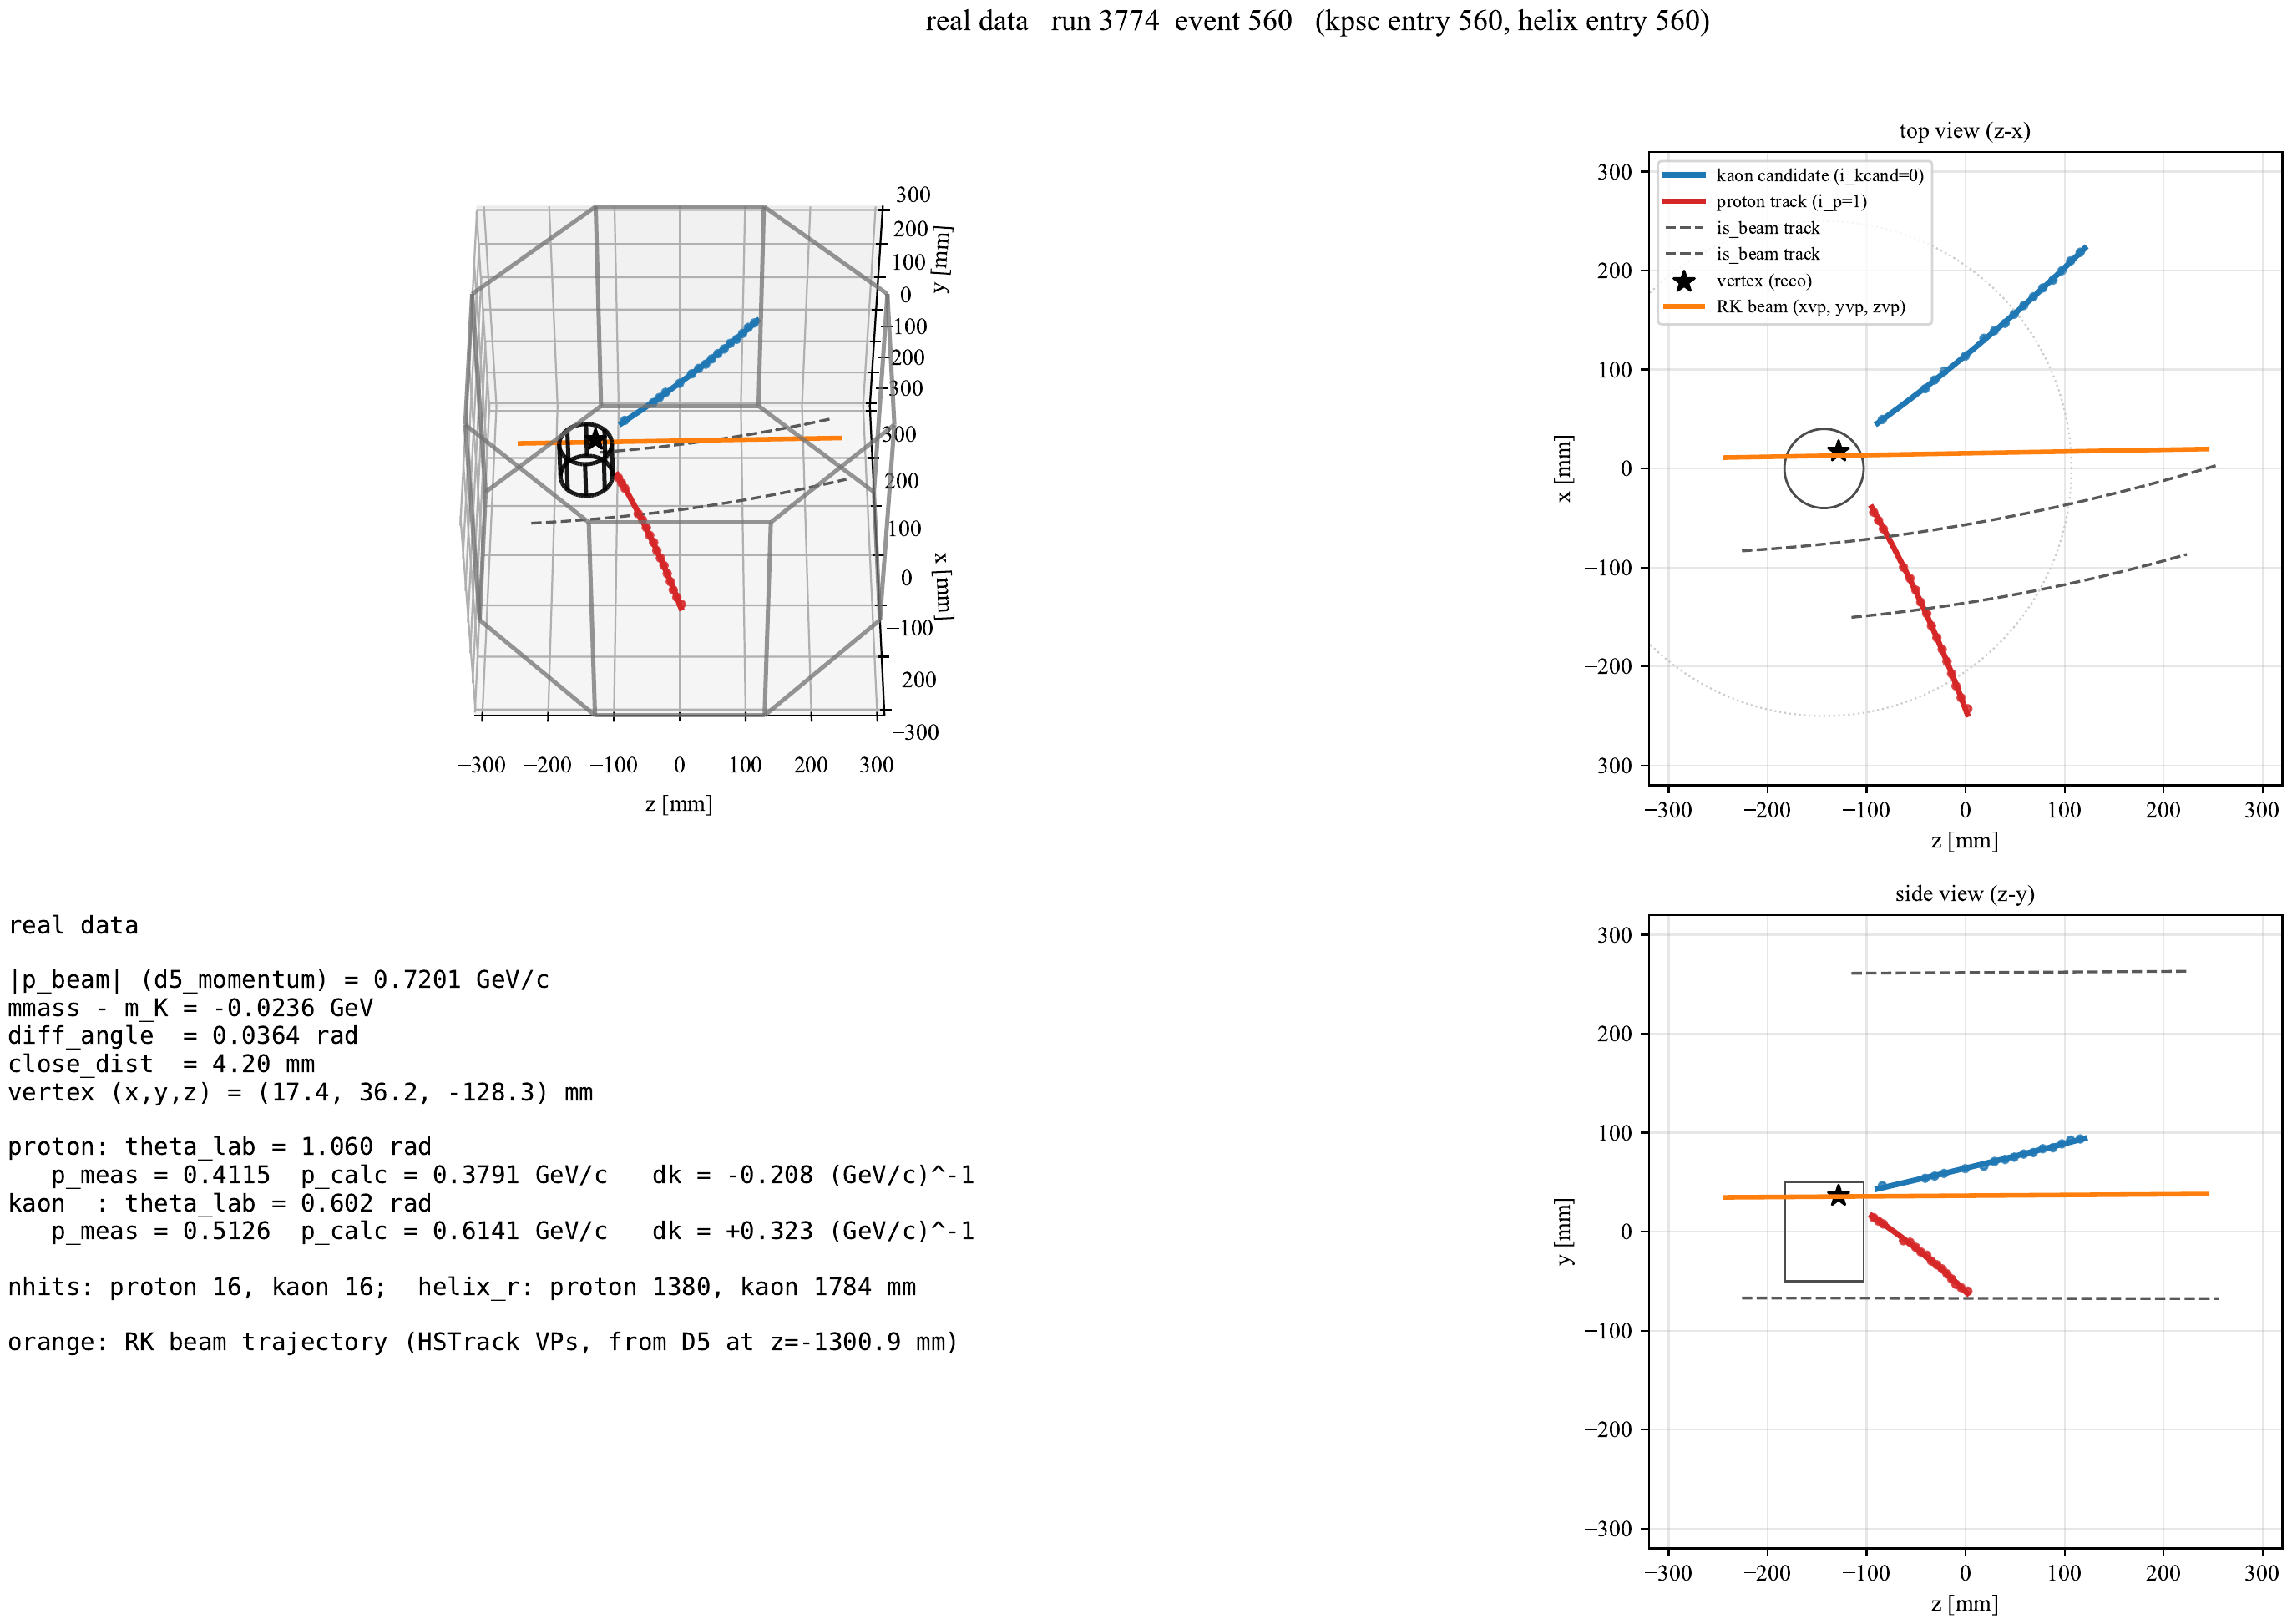
\includegraphics[width=\textwidth]{manual_fig_kpsc_event_display_rk/evdisp_data.png}
\caption{実データ（run 3774）の例。}
\end{figure}
\begin{figure}[H]
\centering
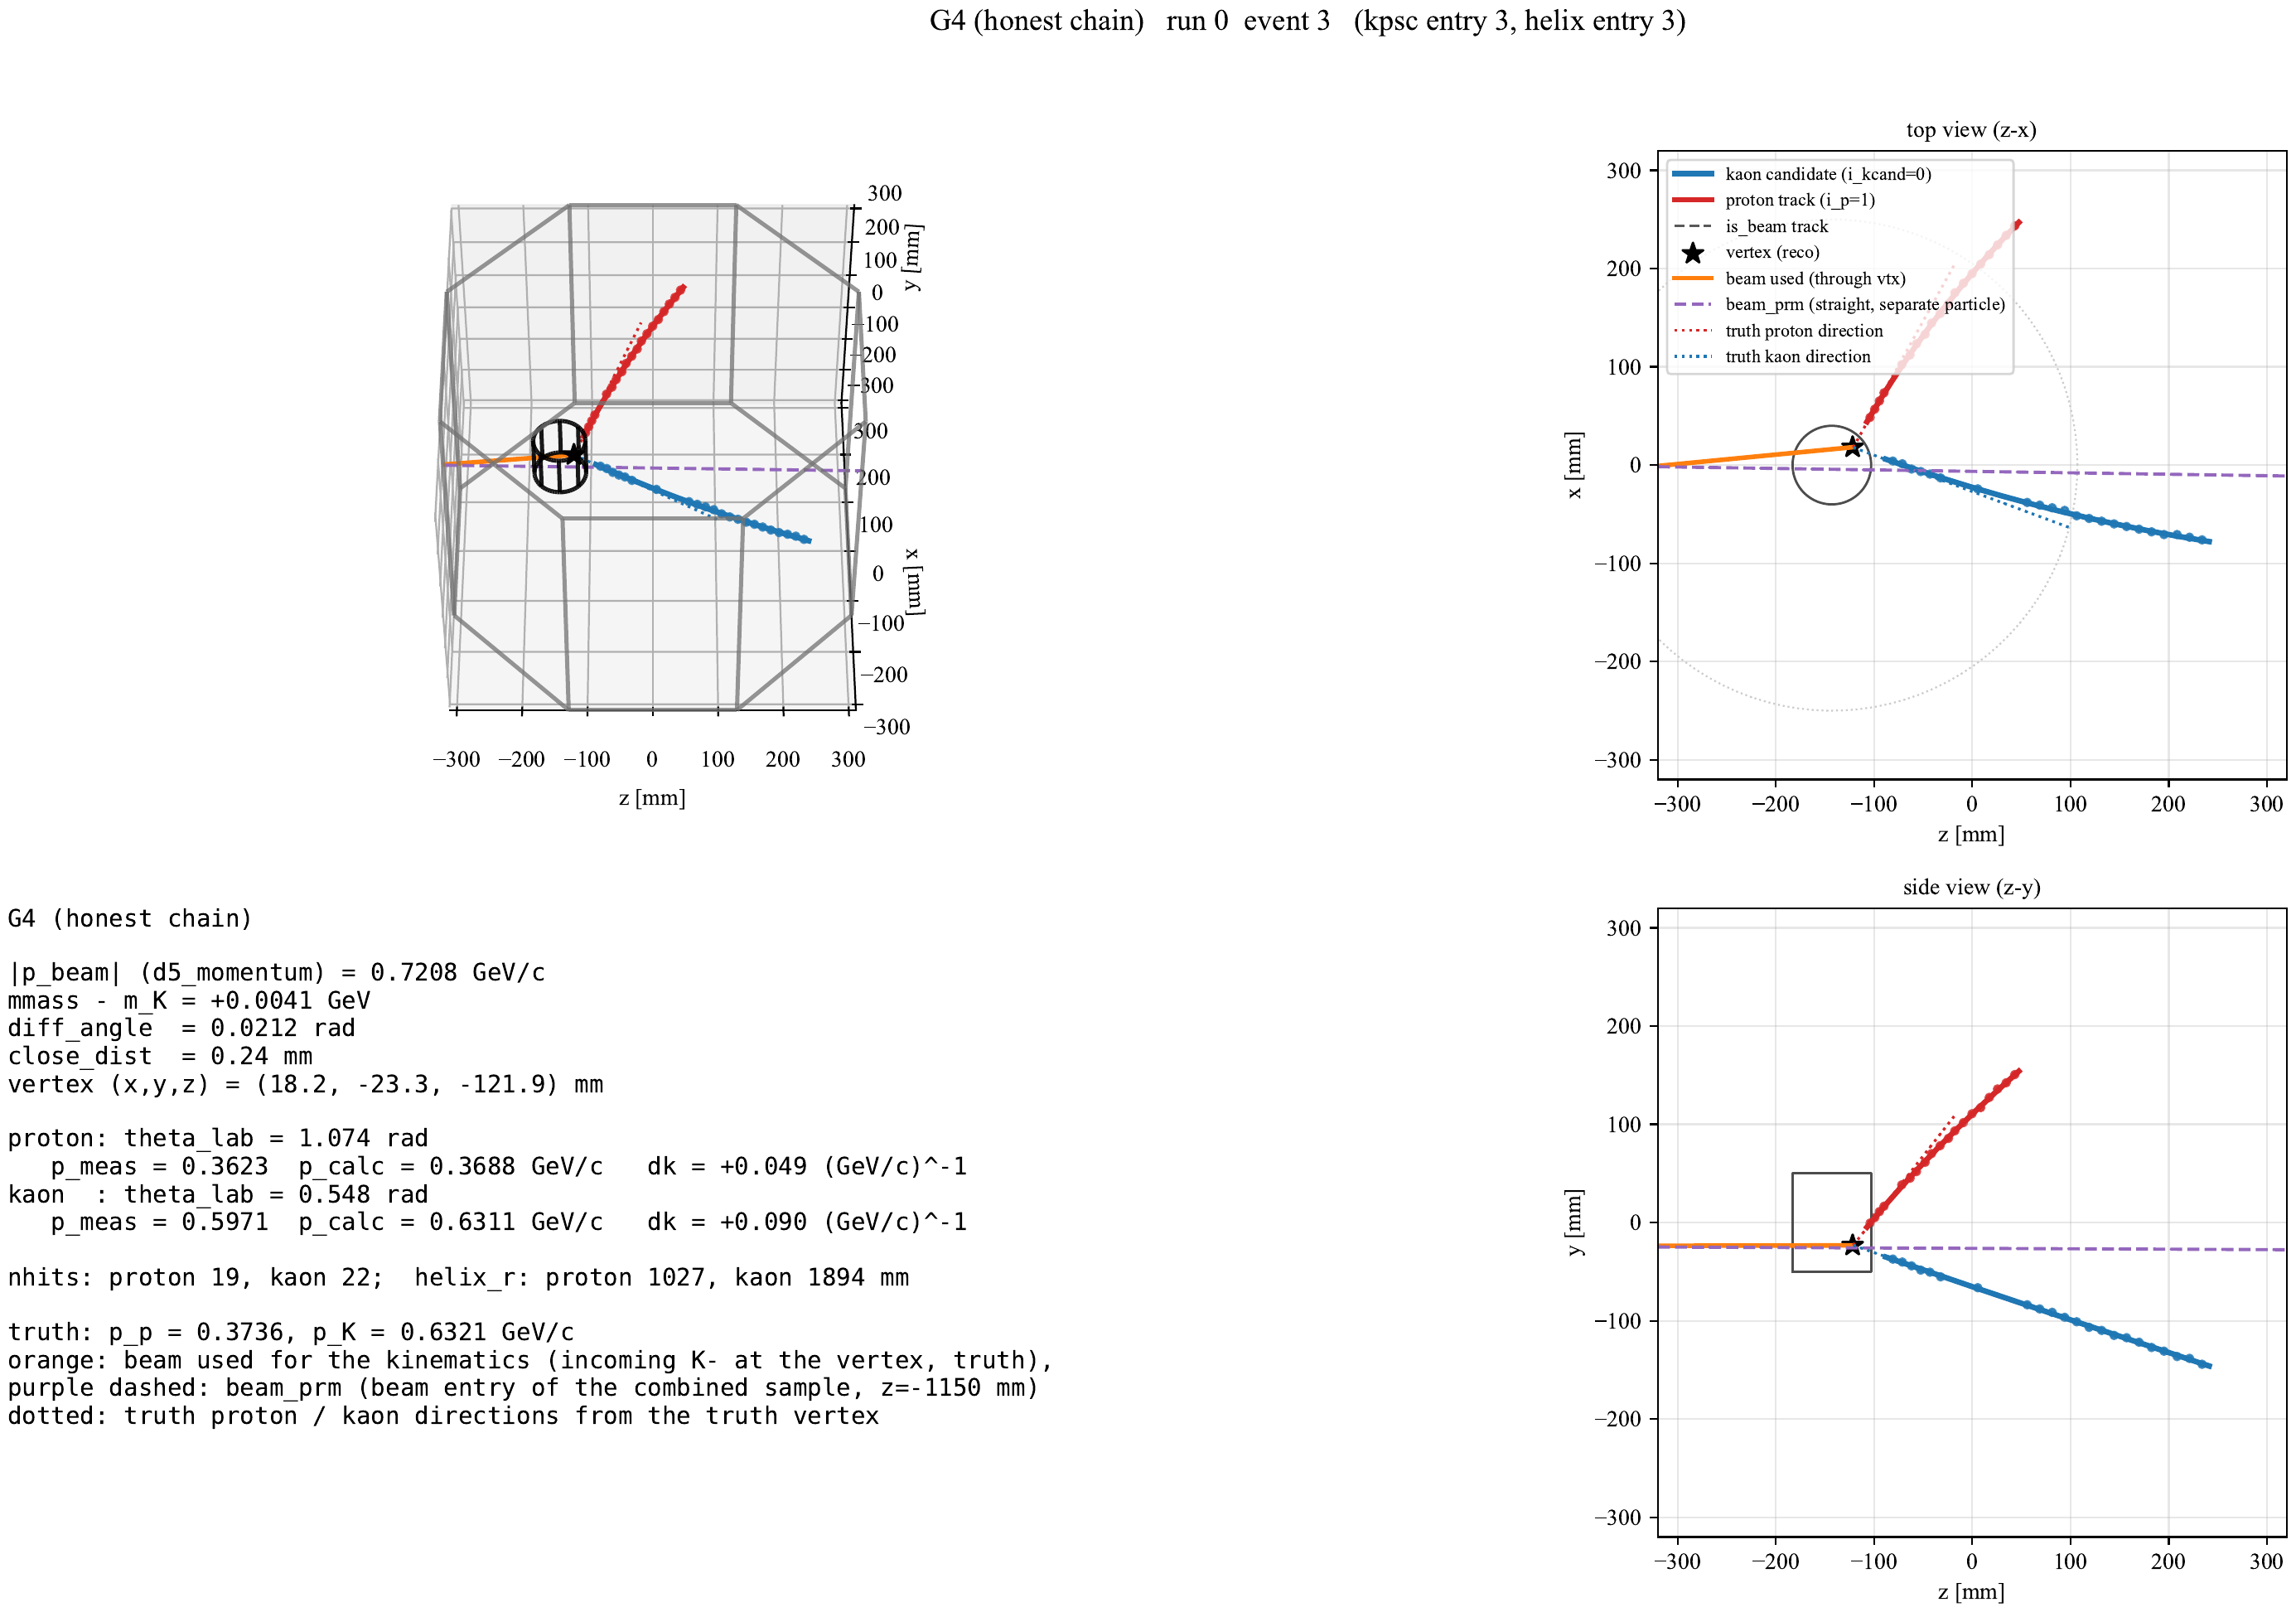
\includegraphics[width=\textwidth]{manual_fig_kpsc_event_display_rk/evdisp_g4.png}
\caption{G4 の例。}
\end{figure}

\section{実行時間とメモリ}
\begin{itemize}
\item 起動時に helix の \texttt{event\_number}（と \texttt{run\_number}）と kpsc のスカラー量を全エントリ読みます。実データ 1 ラン（約 82 万エントリ）で、1 イベントの描画に約 30 秒かかります。大部分はこの読み込みです。
\item 描画するイベントの helix と \texttt{xvp, yvp, zvp} は、そのエントリだけを読みます。
\item \texttt{--n 12} は、実データ 1 ランで約 40 秒、G4（5 万エントリ）で約 10 秒です。
\end{itemize}

\section{Python から使う}
関数 \texttt{main} にコマンドラインと同じ引数のリストを渡せます。
\begin{Verbatim}
import sys; sys.path.insert(0, "/home/had/sryuta/analyzer/JPARC2025E72/myanalysis/macro")
import kpsc_event_display_rk as ed
ed.main(["--helix", "run03774_TPCHelix.root",
         "--kpsc", "run03774_KpScattering_lh2off.root",
         "--run", "3774", "--event", "560", "--out", "ev.png"])
\end{Verbatim}

\end{document}
